

\newpage
\begin{tikzpicture}[scale=0.75,domain=-3:3] 
  \begin{scope}
    \clip (-3,-3) rectangle (3,3);
    \draw[red,very thick,dashed] 
    plot (\x,{(\x)^2}) node [below right] {$y=x^2$};
  \end{scope}
  \draw[->] (-3,0) -- (3,0) node[right] {$x$};  
  \draw[->] (0,0) -- (0,3) node[above] {$y$};  
  \draw ({sqrt(3)},3) node[right] {$\color{blue}x^2$};
  
\end{tikzpicture}
\newpage

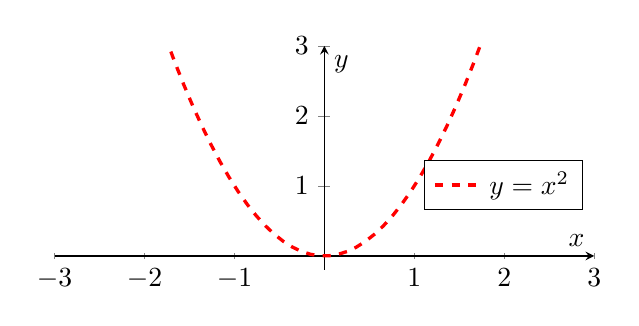
\begin{tikzpicture}
  \begin{axis}[xmin=-3,xmax=3,ymax=3,ymin=-0.2,xlabel = $x$, ylabel=$y$,
    samples=100, axis lines = middle, yscale=0.5]
    \addplot[dashed, very thick,red]{x^2};\addlegendentry{$y=x^2$}
  \end{axis}
\end{tikzpicture}


\newpage

\begin{tikzpicture}[scale=0.5,domain=-4:4]
  \draw[->] (-4.25,0) -- (4.25,0) node[right] {$x$};
  \draw[->] (0,-4) -- (0,4) node[above] {$y$};
  
  \foreach \x in {-4, -3, ..., 4}
  \draw[shift={(\x,0)}] (0pt,2pt) -- (0pt,-2pt) node[below]
  {$\x$};
  
  \foreach \y in {-3,-2,-1,1,2,3}
  \draw[shift={(0,\y)}] (2pt,0pt) -- (-2pt,0pt) node[left] 
  {$\y$};
\end{tikzpicture}

\newpage
\begin{tikzpicture}[scale=0.75,domain=0:2*pi]
  \draw[red,samples=100] plot (\x,{sin(\x r)}) node [below right] {$y=\sin(x)$};
  
  \draw[->] (0,0) -- (7,0) node[right] {$x$};
  
  \draw[->] (0,-2) -- (0,2) node[above] {$y$};
  
  \foreach \x/\xtext in {0/0,{pi/2}/\frac \pi2,pi/\pi,2*pi/2\pi}
  \draw[shift={(\x,0)}] (0pt,2pt) -- (0pt,-2pt) node[above]
  {$\xtext$};
  
\end{tikzpicture}

\newpage
\begin{tikzpicture}
  \begin{axis}[scale=0.75,xlabel = $x$, ylabel=$y$,samples=100, 
    axis lines = middle,domain=0:4.5*pi,
    xtick={0,1.5708,...,15},
    xticklabels={0,$\frac \pi2$,$\pi$,,$2\pi$,,$3\pi$,,$4\pi$},
    title={\textbf{Obr�zek v pgfplots}}
    ]
    \addplot[green,thick] {sin(deg(x))};
    \node[right,red] at (axis cs:6.28,0.5) {Text};
  \end{axis}
\end{tikzpicture}


\newpage

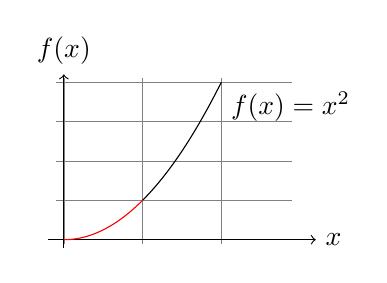
\begin{tikzpicture}[yscale=0.5]
    \draw[very thin,color=gray] (-0.1,-0.1) grid (2.9,4.1);
    \draw[->] (-0.2,0) -- (3.2,0) node[right] {$x$};
    \draw[->] (0,-0.2) -- (0,4.2) node[above] {$f(x)$};

    \draw[domain=1:2] plot (\x,{\x^2}) node[below right] {$f(x) = x^2$};
    \draw[domain=0:1,red] plot (\x,{\x^2}) ;
\end{tikzpicture}

\newpage
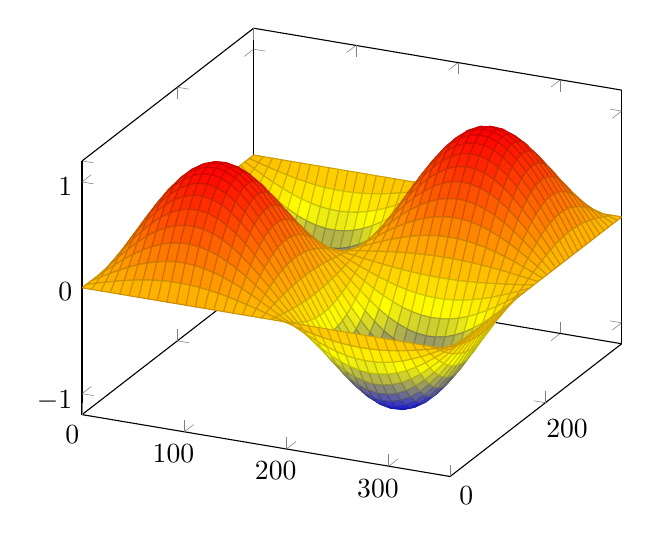
\begin{tikzpicture}
\begin{axis}
\addplot3[surf,domain=0:360,samples=40]
{sin(x)*sin(y)};
\end{axis}
\end{tikzpicture}

\newpage

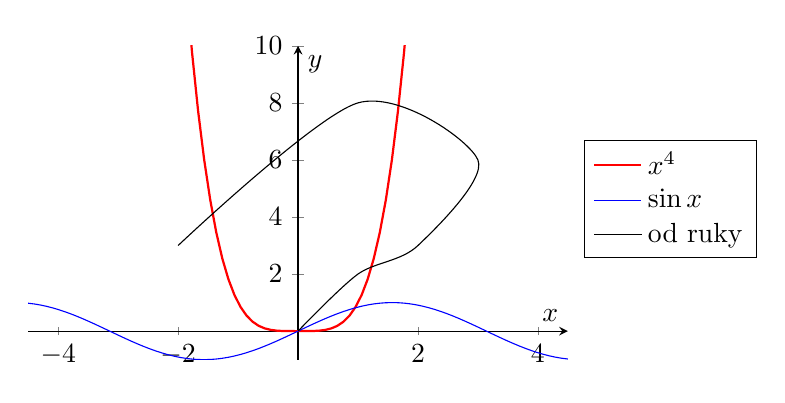
\begin{tikzpicture}
   \begin{axis}[xlabel = $x$, ylabel=$y$, xmin=-4.5, xmax=4.5, 
     ymax=10, yscale=0.7, samples=100, axis lines = middle,
     legend style={
       cells={anchor=west},
       legend pos=outer north east,
     }
     ]
    \addplot[thick, red]{x^4};
    \addlegendentry{$x^4$}
    \addplot[blue]{sin(deg(x))};
    \addlegendentry{$\sin x$}
    \addplot[smooth] coordinates
    {(0,0) (1,2) (2,3) (3,6) (1,8) (-2,3)};
    \addlegendentry{od ruky}
  \end{axis}
\end{tikzpicture}


\newpage

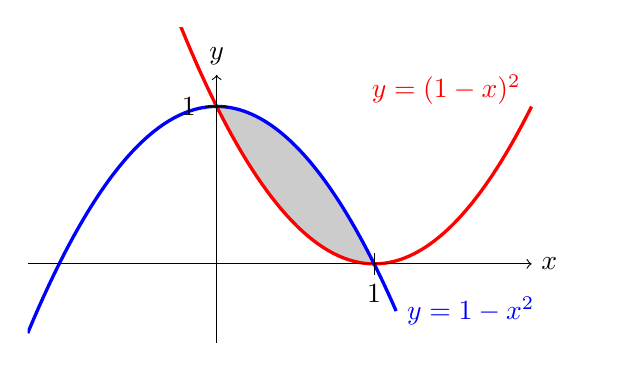
\begin{tikzpicture}[scale=2]
  \clip (-1.2, -0.5) rectangle (2.5, 1.5);
  \fill[gray!40, samples=100] plot[domain=0:1] (\x,{(\x-1)^2}) --  plot[domain=1:0] (\x,{1-(\x)^2}) -- cycle ;
  
  \draw[red,samples=100,domain=-1.2:2,very thick] plot (\x,{(\x-1)^2}) node[left,yshift=6pt] {$y=(1-x)^2$};
  \draw[blue,samples=100,domain=-1.2:1.14,very thick] plot (\x,{1-(\x)^2}) node[right] {$y=1-x^2$};
  
  \draw[->] (-1.2,0) -- (2,0) node[right] {$x$};
  \draw[->] (0,-1.2) -- (0,1.2) node[above] {$y$};
  \draw[shift={(1,0)}] (0pt,2pt) -- (0pt,-2pt) node[below] {$ 1$};
  \draw[shift={(0,1)}] (2pt,0pt) -- (-2pt,0pt) node[left] {$1$};
\end{tikzpicture}

\newpage


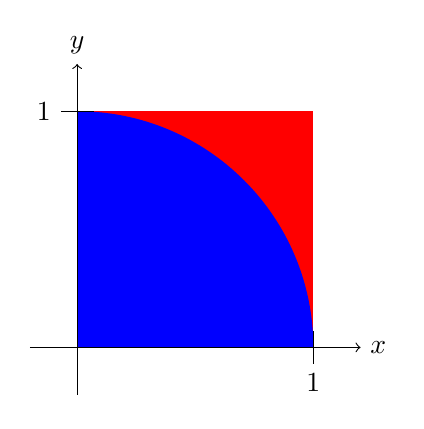
\begin{tikzpicture}[scale=3]
  \fill[fill=red] (0,0) rectangle (1,1);
  \fill[fill=blue] (1,0) arc (0:90:1) -- (0,0) -- cycle;
  \draw[->] (-.2,0) -- (1.2,0) node[right] {$x$};
  \draw[->] (0,-0.2) -- (0,1.2) node[above] {$y$};
  \draw[shift={(1,0)}] (0pt,2pt) -- (0pt,-2pt) node[below] {$ 1$};
  \draw[shift={(0,1)}] (2pt,0pt) -- (-2pt,0pt) node[left] {$1$};
\end{tikzpicture}

\newpage
\usetikzlibrary{calc}
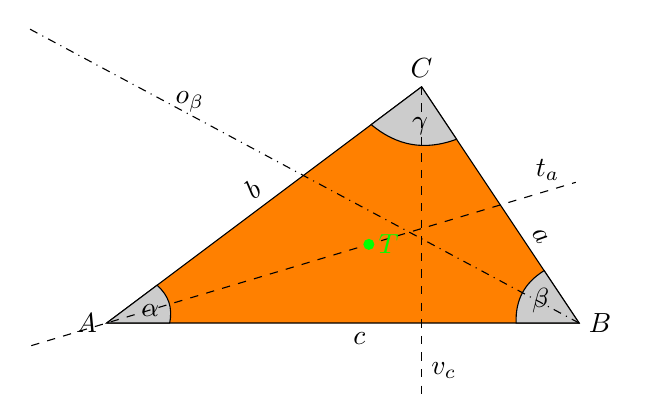
\begin{tikzpicture}[x=1.0cm,y=1.0cm]
  \coordinate (A) at (0,0); 
  \coordinate (C) at (4,3);
  \coordinate (B) at (6,0); 
  \coordinate (D) at ($(B)!0.5!(C)$);   % stred strany a
  \coordinate (E) at ($(A)!(C)!(B)$);   % pata vysky na stranu c
  \coordinate (T) at ($(A)!0.666!(D)$);   % teziste
  \coordinate (p1) at ($(B)!9cm!(C)$);  
  \coordinate (p2) at ($(B)!9cm!(A)$);  
  \coordinate (p3) at ($(p1)!0.5!(p2)$);  % bod kterym prochazi osa uhlu beta
  
  \draw[color=black,fill=orange] 
  (A) node[left] {$A$}
  -- node [sloped, below, xshift=6pt] {$c$} 
  (B) node [right] {$B$}
  -- node [sloped, above, pos=0.33] {$a$}
  (C) node [above] {$C$}
  -- node [sloped, above] {$b$} (A);
  
  \draw[fill=black!20] (B) -- ($(B)!8mm!(C)$) to[bend right] node[right,yshift=-3pt] {$\beta$}
  ($(B)!8mm!(A)$) -- cycle;
  
  \draw[fill=black!20] (A) -- ($(A)!8mm!(C)$) to[bend left] node[left,yshift=-3pt] {$\alpha$}
  ($(A)!8mm!(B)$) -- cycle;
  
  \draw[fill=black!20] (C) -- ($(C)!8mm!(A)$) to[bend right] node[above, xshift=3pt] {$\gamma$}
  ($(C)!8mm!(B)$) -- cycle;

  \draw[color=black,style=dashed, shorten >=-1cm,shorten <=-1cm] (A) -- node [above, pos=1.12] {$t_a$} (D) ; % teznice
  
  \draw[color=black,style=dashed, shorten >=-1cm] (C) -- node [right, pos=1.2] {$v_c$} (E) ; % vyska
  
  \draw[color=black,style=dashdotted] (B) -- node [right, near end] {$o_\beta$} (p3) ;  % osa uhlu
  
  \fill [green] (T) circle [radius=2pt] node [right] {$T$}; % teziste
  
  
\end{tikzpicture}


\newpage

% Export z programu Geogebra
\definecolor{qqzztt}{rgb}{0,0.6,0.2}
\definecolor{qqqqff}{rgb}{0,0,1}
\definecolor{xdxdff}{rgb}{0.49,0.49,1}
\definecolor{uququq}{rgb}{0.25,0.25,0.25}
\usetikzlibrary{arrows}
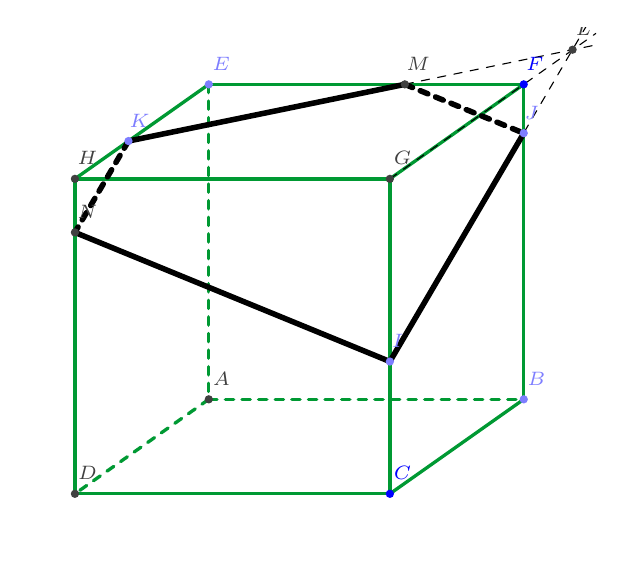
\begin{tikzpicture}[line cap=round,line join=round,>=triangle 45,x=1.0cm,y=1.0cm]
\clip(-2.3,-1.74) rectangle (4.92,4.72);
\draw [line width=1.2pt,dash pattern=on 3pt off 3pt,color=qqzztt] (0,0)-- (4,0);
\draw [line width=1.2pt,color=qqzztt] (4,0)-- (2.3,-1.2);
\draw [line width=1.2pt,color=qqzztt] (2.3,-1.2)-- (-1.7,-1.2);
\draw [line width=1.2pt,dash pattern=on 3pt off 3pt,color=qqzztt] (0,0)-- (-1.7,-1.2);
\draw [line width=1.2pt,color=qqzztt] (0,4)-- (4,4);
\draw [line width=1.2pt,color=qqzztt] (4,4)-- (2.3,2.8);
\draw [line width=1.2pt,color=qqzztt] (2.3,2.8)-- (-1.7,2.8);
\draw [line width=1.2pt,color=qqzztt] (-1.7,2.8)-- (0,4);
\draw [line width=1.2pt,color=qqzztt] (4,4)-- (4,0);
\draw [line width=1.2pt,color=qqzztt] (2.3,2.8)-- (2.3,-1.2);
\draw [line width=1.2pt,color=qqzztt] (-1.7,2.8)-- (-1.7,-1.2);
\draw [line width=1.2pt,dash pattern=on 3pt off 3pt,color=qqzztt] (0,4)-- (0,0);
\draw [dash pattern=on 3pt off 3pt,domain=2.3:4.92] plot(\x,{(--2--1.2*\x)/1.7});
\draw [dash pattern=on 3pt off 3pt,domain=-1.018429561200924:4.92] plot(\x,{(--19.68--1.16*\x)/5.64});
\draw [line width=2pt,dash pattern=on 3pt off 3pt] (2.49,4)-- (4,3.38);
\draw [line width=2pt] (-1.02,3.28)-- (2.49,4);
\draw [line width=2pt] (2.3,0.48)-- (4,3.38);
\draw [line width=2pt,dash pattern=on 3pt off 3pt] (-1.02,3.28)-- (-1.7,2.12);
\draw [line width=2pt] (-1.7,2.12)-- (2.3,0.48);
\draw [dash pattern=on 3pt off 3pt,domain=2.3:4.92] plot(\x,{(-7.99--3.96*\x)/2.32});
\begin{scriptsize}
\fill [color=uququq] (0,0) circle (1.5pt);
\draw[color=uququq] (0.16,0.26) node {$A$};
\fill [color=xdxdff] (4,0) circle (1.5pt);
\draw[color=xdxdff] (4.16,0.26) node {$B$};
\fill [color=qqqqff] (2.3,-1.2) circle (1.5pt);
\draw[color=qqqqff] (2.46,-0.94) node {$C$};
\fill [color=uququq] (-1.7,-1.2) circle (1.5pt);
\draw[color=uququq] (-1.54,-0.94) node {$D$};
\fill [color=xdxdff] (0,4) circle (1.5pt);
\draw[color=xdxdff] (0.16,4.26) node {$E$};
\fill [color=qqqqff] (4,4) circle (1.5pt);
\draw[color=qqqqff] (4.14,4.26) node {$F$};
\fill [color=uququq] (2.3,2.8) circle (1.5pt);
\draw[color=uququq] (2.46,3.06) node {$G$};
\fill [color=uququq] (-1.7,2.8) circle (1.5pt);
\draw[color=uququq] (-1.54,3.06) node {$H$};
\fill [color=xdxdff] (2.3,0.48) circle (1.5pt);
\draw[color=xdxdff] (2.4,0.74) node {$I$};
\fill [color=xdxdff] (4,3.38) circle (1.5pt);
\draw[color=xdxdff] (4.1,3.64) node {$J$};
\fill [color=xdxdff] (-1.02,3.28) circle (1.5pt);
\draw[color=xdxdff] (-0.88,3.54) node {$K$};
\fill [color=uququq] (4.62,4.44) circle (1.5pt);
\draw[color=uququq] (4.76,4.7) node {$L$};
\fill [color=uququq] (2.49,4) circle (1.5pt);
\draw[color=uququq] (2.66,4.26) node {$M$};
\fill [color=uququq] (-1.7,2.12) circle (1.5pt);
\draw[color=uququq] (-1.54,2.38) node {$N$};
\end{scriptsize}
\end{tikzpicture}


\newpage
\usetikzlibrary{calc,intersections,through,backgrounds}
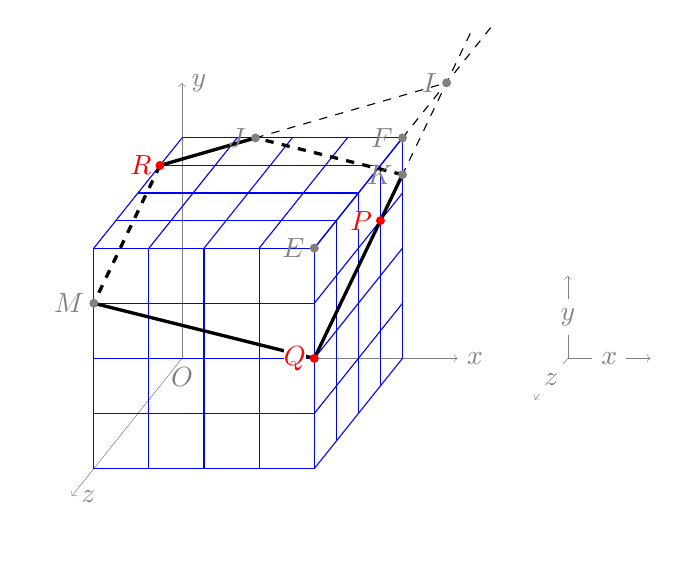
\begin{tikzpicture}[z={(-.4,-0.5)},scale=0.7]
\coordinate (O) at (0,0,0);

% osy
\begin{scope}[gray, very thin,->]
  \draw[->] (7,0,0) -- node[fill=white] {$x$} ++ (1.5,0,0);
  \draw[->] (7,0,0) -- node[fill=white] {$y$} ++ (0,1.5,0);
  \draw[->] (7,0,0) -- node[fill=white] {$z$} ++ (0,0,1.5);

  \draw (O) node [below] {$O$} --(5,0,0) node[right] {$x$};
  \draw (O) -- (0,5,0) node[right] {$y$};
  \draw (O) -- (0,0,5) node[right] {$z$};
\end{scope}

\clip (0,0,7) rectangle (7,6,0); % orez obrazku
% krychle
\begin{scope}[blue]
  \foreach \x in{0,...,4}
  {   \draw (0,\x ,4) -- (4,\x ,4);
    \draw (\x ,0,4) -- (\x ,4,4);
    \draw (4,\x ,4) -- (4,\x ,0);
    \draw (\x ,4,4) -- (\x ,4,0);
    \draw (4,0,\x ) -- (4,4,\x );
    \draw (0,4,\x ) -- (4,4,\x );
  }
\end{scope}

\foreach \x/\a in {P/{4,3,1}, Q/{4,2,4}, 
  R/{0,4,1},  E/{4,4,4}, F/{4,4,0}}
{\coordinate (\x) at (\a);}  % definice bodu

\draw[name path=line 1,dashed] (P) -- ($(Q)!3!(P)$); % prodlouzeni usecky PQ
\draw[name path=line 2,dashed] (F) -- ($(E)!3!(F)$); % prodlouzeni usecky FE
\path[name intersections={of=line 1 and line 2,by=I}]; % prusecik

\path[name path=line 4] (0,4,0) -- (F); % pojmenovani usecky
\path[name path=line 3] (R) -- (I); % pojmenovani usecky
\path [name intersections={of=line 3 and line 4,by=J}]; % prusecik

\path[name path=line 5] (4,0,0) -- (4,4,0); % pojmenovani hrany krychle
\path[name intersections={of=line 5 and line 1,by=K}]; % prusecik

\path[name path=line 6] (R) -- +($5*(Q)-5*(P)$); % Rovnobezka bodem R, smer vektoru PQ, petinasobek delky
\path[name path=line 7] (0,0,4) -- (0,4,4); % pojmenovani hrany krychle
\path[name intersections={of=line 6 and line 7,by=M}]; % prusecik

\begin{scope}[very thick] % vykresleni rezu
  \draw (M) -- (Q) -- (K);
  \draw[dashed](K)--(J);
  \draw (J)--(R);
  \draw[dashed] (R) --(M);
\end{scope}
\draw[dashed] (J)--(I);

\foreach \x in {E,F,I,J,K,M} {\draw[fill,gray] (\x) circle [radius=2pt] node [above, left] {$\x$};} 

\foreach \x in {P,Q,R} {\draw[fill,red] (\x) circle [radius=2pt] node [inner sep = 0pt,left,fill=white,shift={(-.1,0)}] {$\x$};} 

\end{tikzpicture}

\newpage

\def\ymax{2}
\def\ymin{-2}
\def\xmax{2}
\def\xmin{-3}
\def\xsize{0.6}
\def\ysize{0.3}
\colorlet{color1}{brown}
\colorlet{color2}{blue}
\colorlet{color3}{green}
\usetikzlibrary{arrows}
\begin{tikzpicture}[scale=0.8]
  \footnotesize
  \begin{scope}
    \clip (\xmin,-2) rectangle (\xmax,\ymax);
    \draw[fill=color3] plot[domain=\xmin:-3/4] 
    (\x,{\x-1+sqrt(1-4*\x)}) -- (-3/4,1/4) -- (-3/4,-3/4) -- (\xmin,\xmin);
    \draw[] (\xmin,\xmin) -- (\ymax,\ymax);
  \end{scope}
  
  \draw[fill=color2] (1/4,\ymax) -- (1/4,1/4) -- (\ymax,\ymax);
  \draw[fill=color1] (-3/4,-3/4) -- (-3/4,1/4) -- (1/4,1/4) --(-3/4,-3/4) ;
  
  \draw (\xmax,\xmax)  node [anchor = south west]{$Q_*=Q^*$};
  
  \draw[arrows={-angle 45}] (\xmin,0) -- (\xmax,0) node[right] {$Q_*$};
  \draw[arrows={-angle 45}] (0,\ymin) -- (0,\ymax) node[above] {$Q^*$};
  \draw[red, very thick] plot[domain=\xmin:-3/4] (\x,{\x-1+sqrt(1-4*\x)});
  
  \draw[shift={(-0.8,0)}] (0pt,2pt) -- (0pt,-2pt) node[below] {$-\frac 34$};
    \draw[shift={(1/4,0)}] (0pt,2pt) -- (0pt,-2pt) node[below] {$\frac 14$};
  
  \def\barva{yellow}
  \draw[shift={(0,-0.8)}] (\xmin,0) node[anchor=east]
  {\hbox {\hss \colorbox{\barva}{$Q^*=Q_*-1+\sqrt{1-4Q_*}$}}};

  \def\barva{green!50!yellow}
  \draw [shift={(1,1)}] (\xmin,0) node[anchor=east]{\hbox {\hss \colorbox{\barva}{$
        \begin{aligned}
          Q_*&=\frac 12\left(-t-\sqrt{2t}\right)\\
          Q^*&=\frac 12\left(-t+\sqrt{2t}\right), t\in\left(\frac  12,\infty\right)
        \end{aligned}
        $}}};
\end{tikzpicture}


\newpage

\pgfmathdeclarefunction{gauss}{2}{%
  \pgfmathparse{1/(#2*sqrt(2*pi))*exp(-((x-#1)^2)/(2*#2^2))}%
}

\begin{tikzpicture}[scale=0.8]
\begin{axis}[
  no markers, domain=0:10, samples=100,
  axis lines*=left, xlabel=$x$, ylabel=$y$,
  every axis y label/.style={at=(current axis.above origin),anchor=south},
  every axis x label/.style={at=(current axis.right of origin),anchor=west},
  height=5cm, width=12cm,
  xtick={4,6.5}, ytick=\empty,
  enlargelimits=false, clip=false, axis on top,
  grid = major
  ]
  \addplot [fill=cyan!20, draw=none, domain=0:5.96] {gauss(6.5,1)} \closedcycle;
  \addplot [very thick,cyan!50!black] {gauss(4,1)};
  \addplot [very thick,cyan!50!black] {gauss(6.5,1)};


  \draw [yshift=-0.6cm, latex-latex](axis cs:4,0) -- node [fill=white] 
  {$1.96\sigma$} (axis cs:5.96,0);
\end{axis}

\end{tikzpicture}

\newpage

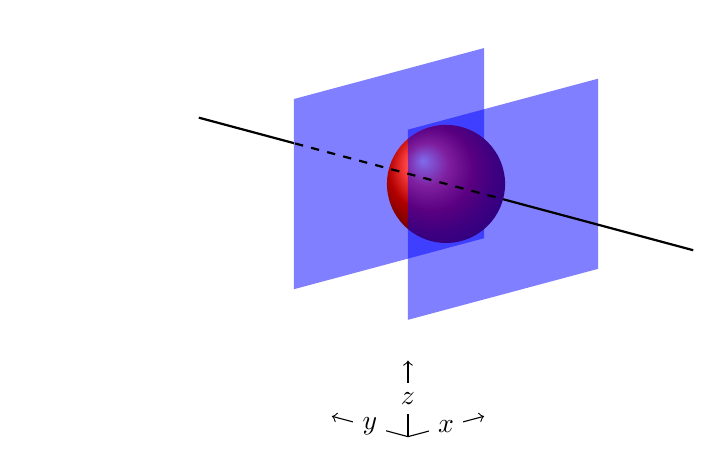
\begin{tikzpicture}[x={(0.966cm,0.259cm)},y={(-0.966cm,0.259cm)},z={(0.0cm,0.966cm)},scale=0.5]
\draw[->] (-2,-2,-2) -- node[fill=white] {$x$} ++ (2,0,0);
\draw[->] (-2,-2,-2) -- node[fill=white] {$y$} ++ (0,2,0);
\draw[->] (-2,-2,-2) -- node[fill=white] {$z$} ++ (0,0,2);

\begin{scope}
    \clip (0,3,0) -- (0,3,5) -- (0,10,5) -- (0,10,0) -- cycle;
    \draw[thick] (2.5,8,2.5) -- (2.5,3,2.5);
\end{scope}

\fill[opacity=0.5,blue] (0,3,0) -- (5,3,0) -- (5,3,5) -- (0,3,5) -- cycle;
\shade[ball color=red] (2.5,1.5,2.5) circle (1.5*1cm);
\fill[opacity=0.5,blue] (0,0,0) -- (5,0,0) -- (5,0,5) -- (0,0,5) -- cycle;

\begin{scope}
    \clip (0,0,0) -- (2.5,0,0) -- (2.5,0,5) -- (2.5,3,5) -- (0,3,5) -- (0,3,0) -- cycle;
    \draw[thick, dashed] (2.5,8,2.5) -- (2.5,0,2.5);
\end{scope}

\draw[thick] (2.5,0,2.5) -- (2.5,-5,2.5);

\end{tikzpicture}

\newpage

\end{document}
